%%%%%%%%%%%%%%%%%%%%%%%%%%%%%%%%%%%%%%%%%%%%%%%
% IOE Graduate Conference, 2019
% Working Paper Template
% Version 4.0
%
% Original author:
% Jayandra Raj Shrestha (jayandra@ioe.edu.np)
%%%%%%%%%%%%%%%%%%%%%%%%%%%%%%%%%%%%%%%%%%%%%%%

\documentclass[fleqn, 11pt, twoside]{IOEGC2019}

\usepackage{float}  % To force placing figures and tables at desired location

% metadata for pdf file, visible from File -> Properties dialog in Adobe reader
% also required for titles when viewed in web browser
\hypersetup
{
    pdftitle    = {Preparing Your Paper in LaTeX for IOEGC-2019},
    pdfsubject  = {IOE Graduate Conference, 2019},
    pdfauthor   = {	Jayandra Raj Shrestha, 
					Arun Kumar Timalsina, 
					Binod Kumar Bhattarai },    
    pdfkeywords = {IOE Graduate Conference, LaTeX, Template}
}

\PaperTitle{Preparing Your Paper in \LaTeX\  for IOEGC-2019}

% Author Names -- Do not include titles like Prof., Dr., Mr. etc.
% Replace with enough placeholder text in initial submission for Blind Review
% Replace with actual names in the final submission after the review is over
\Authors{
	Jayandra Raj Shrestha \textsuperscript{a}, 
	Binod Kumar Bhattarai \textsuperscript{b}, 
	Arun Kumar Timalsina  \textsuperscript{c}
} 

% Do not include your real affiliations or emails, put some enough random text 
% as placeholder in the initial submission for "Blind Review"
\affiliation{
	\textsuperscript{a, b}
	\textit{Department of Applied Sciences, Pulchowk Campus, IOE, TU, Nepal}
}

\affiliation{
	\textsuperscript{c}
	\textit{Department of Electronics and Computer Engineering, 
			Pulchowk Campus, IOE, TU, Nepal}
} 

\affiliation{\textbf{Corresponding Email}: 
	\textsuperscript{a} jayandra@ioe.edu.np, 
	\textsuperscript{b} binod.bhattarai@ioe.edu.np,
	\textsuperscript{c} t.arun@ioe.edu.np
} 


\Abstract{
	This is a working template for the research paper to be presented at the IOE
	Graduate Conference - 2019. The template has been typeset in \LaTeX. 
	You have to replace certain sections of this template by your content and 
	produce a pdf file as final output. Format for different types of elements 
	that could occur in the paper are already defined in this template. 
	The authors are to strictly follow the style/formatting as defined in this 
	template for consistencies in a single paper and across different papers.
	The contents of the paper appears in a two column format, with an exception 
	of the paper title, author names, affiliations, abstract and keywords. 
	Your paper should be limited to 8 pages and abstract should not exceed 
	300 words. Each of the keywords need to be separated by -- 
	as given in the example below.
}

% If you don't have any keyword simply remove the text between the curly braces
% But DO noT remove the \Keywords command
\Keywords{IOE Graduate Conference -- \LaTeX\ -- Template} 



\begin{document}
\maketitle
\thispagestyle{firstpage} 


\section{Introduction}              
In the past, the papers for IOE Graduate Conference were submitted as Microsoft 
Word document. Although standard templates were created for the submission, 
there used to be a lot of technical problems in the submitted documents. Only a 
few papers seemed to follow proper guidelines. This resulted in difficulty in 
compiling the final conference proceeding. To overcome this, the IOE Graduaet 
Conference has been using \LaTeX\ as the standard and only tool for preparing 
the manuscript, starting from the year 2015. In word processing softwares like 
Microsoft Word, it is very likely that people create unorganized document, 
whereas in typesetting software environment like \LaTeX, one has to create a 
document in an organized fashion. 

On the other hand, \LaTeX\ is being adapted as the standard tool for producing 
technical documents by most of the top class universities and institutions. 
This means that if the graduate students do not learn \LaTeX\ at the right time,
they will poise some limitations on themselves. So, it should be taken as an 
opportunity to learn \LaTeX. A lot of resources for learning \LaTeX\ can be 
found online. It would take 10--20 hours of learning for getting started with 
\LaTeX\ and would be beneficial for life long.


\section{What is \LaTeX?} \label{sec:whatis}
\LaTeX{} is a document preparation system for the \TeX{}
typesetting program. It offers programmable desktop publishing features and 
extensive facilities for automating most aspects of typesetting and desktop  
publishing, including numbering and cross-referencing,
tables and figures, page layout, bibliographies, and much more. 

\begin{itemize}[noitemsep]
	\item A family of programs designed to produce \\publication-quality typeset
		documents.
	\item Particularly good at working with mathematical symbols.
	\item WYSIWYM\footnote{What You See Is What You Mean} rather than 
		WYSIWYG\footnote{What You See Is What You Get}.
\end{itemize}

The history of LaTeX begins with a program called \TeX. In 1978, a computer 
scientist by the name of \textbf{Donald Knuth} grew frustrated with the mistakes
that his publishers made in typesetting his work. He decided to create a 
typesetting program that everyone could easily use to typeset documents, 
particularly those that include formulae, and made it freely available. 

Knuth's product is an immensely powerful program, but one that does focus
very much on small details. A mathematician and computer scientist by the
name of Leslie Lamport wrote a variant of \TeX\ called \LaTeX\ that focuses on
document structure rather than such details.


\section{Getting the \LaTeX\ Software }\label{sec:getting}
There are two major standard distributions of \LaTeX:
\begin{itemize}[noitemsep]
	\item TeXLive \\ \texttt{\small{https://www.tug.org/texlive/}}
	\item MikTeX \\ \texttt{\small{https://miktex.org/}}
\end{itemize}

These are freely downloadable from the internet. TeXLive works in all the major 
PC platforms like Windows, Unix, Linux, and Mac. Whereas, MikTeX is for Windows 
only. When you install these, you also get the TeXWorks editor as your frontend.
More than a dozen other frontend GUIs are available for \LaTeX. 
Some of these are:

\begin{itemize}[noitemsep]
	\item TeXMaker \\ \texttt{\small{http://www.xm1math.net/texmaker/}}
	\item TeXnic Center\\ \texttt{\small{http://www.texniccenter.org/}}
\end{itemize}


\section{Template Structure} \label{sec:struct}
This \LaTeX\ template resides on a folder with the following files/folder:
\begin{description}
	\item[article.tex]		The main \LaTeX\ source file of this document. 
		Working Example on using the template with some description.
	\item[article.pdf]		Produced by compiling article.tex.
	\item[pagenum.tex]		Contains the code for starting page number which 
							will be edited during final compilation.
	\item[IOEGC2019.cls] 	\LaTeX\ class file for managing the styles and 
		formats of the document. Prohibited to edit.
	\item[refs.bib] 	File for placing the bibliography data in BibTeX format.
	\item[Graphics] 		Folder for keeping all the final graphics files 
							(.jpg, .png, etc.) used in the document. 
	\item[Assets]   		Folder for keeping all the codes/source files 
							(.xls, .xlsx, .m, etc.) used to generate graphs. 
\end{description}


\section{Sections}
Paragraphs within a document can be separated just by leaving one blank line 
between them.

\LaTeX\ supports section headings upto 3 levels via the following commands:

\begin{itemize}[noitemsep]
	\item \verb+\section{...}+
	\item \verb+\subsection{...}+
	\item \verb+\subsubsection{...}+
\end{itemize} 

These have been illustrated properly in section \ref{sec:lists} of this example.
You can use their starred variants given below to suppress section numbering 
which has been demonstrated in the \emph{Acknowledgment} section.

\begin{itemize}[noitemsep]
	\item \verb+\section*{...}+
	\item \verb+\subsection*{...}+
	\item \verb+\subsubsection*{...}+
\end{itemize} 


\section{Typesetting Mathematics}
\LaTeX\ has very rich features for typesetting mathematics. Please refer to 
\LaTeX\ and AMSmath manuals or online resources for further information. 
Here are a few examples.

The formula given in equation \ref{eq:quad} can be used to determine the roots 
of a quadratic equation of the form: $$ax^2+bx+c=0$$
Here, $a$, $b$, and $c$ are constants/coefficients and $x$ is a variable.

Numbered equation:
\begin{equation}
	x= \frac{-b\pm \sqrt{ b^2-4ac}}{2a}
	\label{eq:quad}
\end{equation} 

Equation without a number
\begin{equation*}
	x = \frac{-b\pm \sqrt{ b^2-4ac}}{2a}
\end{equation*} 

\section{Creating Tables}
Table \ref{tbl:capacity} is an example of a simple table in \LaTeX. To create 
complex tables, please refer to \LaTeX\ manuals or online resources. Use 
\verb+\begin{table*}+ to take up the entire page width. However, the use of 
tables spanning the entire page width is discouraged as it needs extra caution.

\begin{table}[H]
	\caption{No. of papers presented in IOEGC}
	\label{tbl:capacity}
	\centering
	\begin{tabular}{|c|l|c|} %three columns: left, center, center aligned
		\hline
		SN & Year & No. of papers \\
		\hline
		1 & 2013 & 42	\\
		2 & 2014 & 79	\\
		3 & 2015 & 46	\\
		4 & 2016 & 49	\\
		5 & 2017 & 83 	\\
		\hline
		 & Total & 299 	\\
		\hline
	\end{tabular}
\end{table}


\section{Placing Figures} \label{sec:figures}
One can generate technical graphs or diagrams from \LaTeX\ also, but this 
requires another level of expertise. Another alternate is to use R-programming 
code to generate graphs on the fly thus producing reproducible documents, 
which requires S-Weave. However, it is very common to include figures generated 
from other sources or programs. Here are a few examples on placing figures with 
proper captioning and label for cross referencing. The most suitable format for 
figure files to produce final output in raster format as pdf are:

\begin{enumerate}[noitemsep]
	\item PNG
	\item PDF
	\item JPG
\end{enumerate}

\begin{figure}[H]\centering
	% Remove fbox if you donot require a bounding box for the image
	\fbox{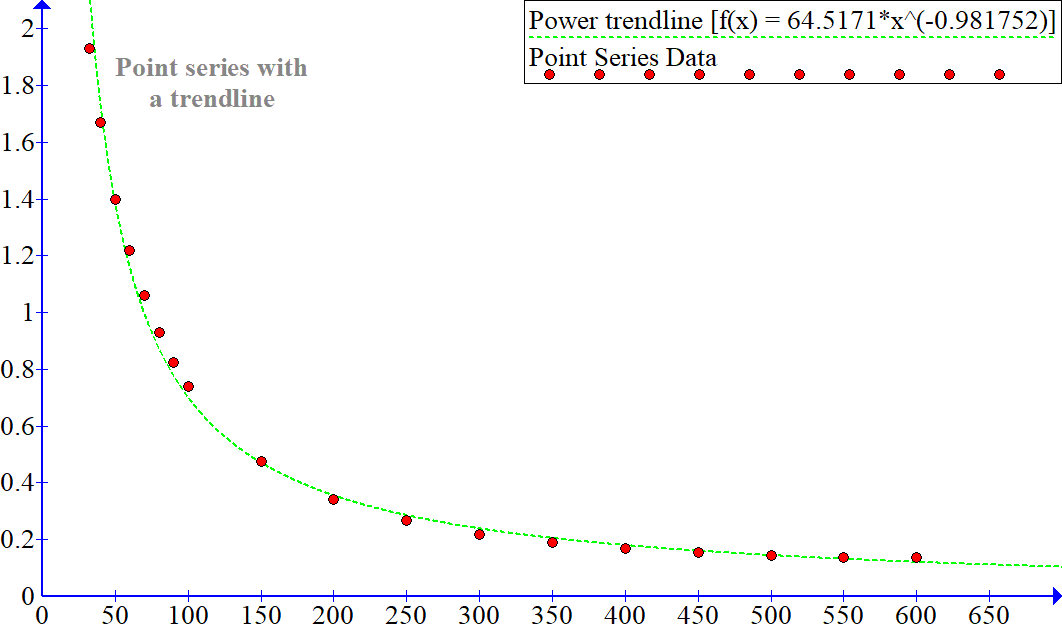
\includegraphics[width=0.95\linewidth]{curve}}
	\caption{Figure taking up 95\% width of the column}
	\label{fig:graph-1}
\end{figure}

% Using \begin{figure*} makes the figure take up the entire width of the page
% But be careful, the figure always comes at the top of the page ... 
% so it may appear on the next available page
\begin{figure*}[hbt]\centering
	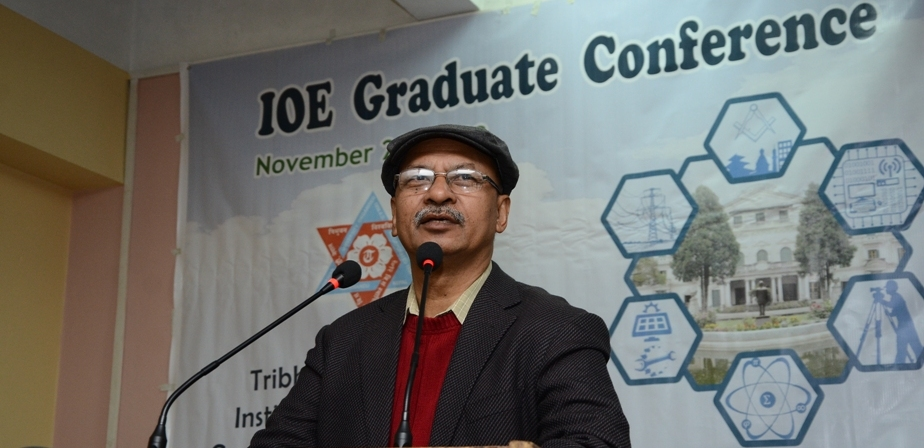
\includegraphics[width=\linewidth]{prof_ale}
	\caption{Placing a wide picture (Discouraged! as it always appears at the 
			 top of a page.)}
	\label{fig:ale-sir}
\end{figure*}

Figure~\ref{fig:graph-1} takes up 95\% of the width of a column and 
Figure~\ref{fig:ale-sir} takes the width of the entire width of the page.

%forcing a column break
%\vfill\null

\section{Lists} \label{sec:lists}

\subsection{Simple Lists}
Simple Bulleted and Numbered lists have already been presented in 
Section~\ref{sec:getting} and Section~\ref{sec:figures} respectively.

\subsection{Nested Lists}
Lists can be nested upto three levels in \LaTeX.

\subsubsection{Numbered Nested List}
Here is a nested numbered list:

\begin{enumerate}
  \item Fruits
    \begin{enumerate}
      \item Apple
      \item Orange
    \end{enumerate}
  \item Vegetables
    \begin{enumerate}
      \item Spinach
      \item Carrot
    \end{enumerate}
\end{enumerate}

\subsubsection{Bulleted Nested List}
Here is a nested bulleted list:

% [noitemsep] removes whitespace between the items for a compact look
\begin{itemize}[noitemsep] 
  \item Fruits
    \begin{itemize}[noitemsep] 
      \item Apple
      \item Orange
    \end{itemize}
  \item Vegetables
    \begin{itemize}[noitemsep] 
      \item Spinach
      \item Carrot
    \end{itemize}
\end{itemize}

\subsubsection{Mixed Nested List}
Here is a mixed nested list:
\begin{enumerate}[noitemsep]
  \item Fruits
    \begin{itemize}[noitemsep] 
      \item Apple
      \item Orange
    \end{itemize}
  \item Vegetables
    \begin{itemize}[noitemsep] 
      \item Spinach
      \item Carrot
    \end{itemize}
\end{enumerate}


\subsection{Description List}
This is for dictionary-like word and description list.
\begin{description}
  \item[Word] Definition ...
  \item[Concept] Explanation ...
  \item[Idea] Text ...
\end{description}


\section{Paragraphs with heading}

\paragraph{Hello} Place your paragraph heading inside the curly braces and your 
paragraph text here.


\section{Referencing}
The list of references should be produced using BibTeX. The BibTeX entries 
should be placed in the "refs.bib" file. Please refer BibTeX manuals or online 
resources on creating bibliography databases using BibTeX and citation. You can 
easily create bibliography database files using the GUIs like TeXMaker or JabRef. 
You can even search for BibTeX entries for a majority of publications at Google 
Scholar in the following url: 

\url{http://scholar.google.com}

Examples: This is citation one\cite{lamport1994} and these are two citations in 
one \cite{oetiker2001not, kopka1995guide}.


\section{Compilation} \label{sec:compile}
Since, this template contains citations and cross referencing along with 
reference list generated via BibTeX, the \LaTeX\ source file should be processed
four times in the following sequence to generate the final pdf output.
\begin{enumerate}
	\item PDFLatex
	\item BibTeX
	\item PDFLatex
	\item PDFLatex
\end{enumerate}

Do not worry, if there is an extra blank page at the end of the paper, this is 
an intended behavior. It happens to make the number of pages of the paper even, 
if the paper ends in an odd-numbered page. This is to make sure that every other
article always starts with an odd-numbered page.


\section{Submission} \label{sec:submit}
Before submitting the paper, the source file must be compiled without any error. 
The files that need to be submitted are:
\begin{itemize}[noitemsep]
\item article.tex
\item article.pdf
\item pagenum.tex
\item refs.bib 
\item IOEGC2019.cls
\item Graphics folder 
\item Assets folder 
\end{itemize}
All these should be placed in compressed / zipped folder and submitted 
electronically.

\section{Review}
Your paper will be peer reviewed in blind by expert(s) before the conference. 
Comments may be provided in the submitted pdf file. You have to re-submit your 
paper by recompiling the \LaTeX\ source file as described in 
section~\ref{sec:compile} and submit as described in section \ref{sec:submit}.

\phantomsection
\section*{Still Having Problem?} 
\addcontentsline{toc}{section}{Problem?} 
There are a lot of online tutorials on \LaTeX\ available for free download. 
One of them being \textit{LaTeX Tutorials -- A Primer} by Indian \TeX\ Users 
Group \cite{ltxprimer}.

Further, there are websites like \url{sharelatex.com}, \url{overleaf.com}, etc.,
 which are very helpful
in finding out how to perform a specific task in \LaTeX\ .

If you still face technical problems in compiling your document in \LaTeX\ using
this template, please feel free to contact the primary author of this template 
via the following email address:

\centerline{\url{jayandra@ioe.edu.np}}

\section*{Future Enhancements}
\addcontentsline{toc}{section}{Future Enhancements} 
Lately, there has been a lot of demand for the creation of reproducible 
documents in research. One of the alternates in producing publication quality 
reproducible documents is the combination of \LaTeX\ and R-programming called 
S-weave. 

In the near future, IOEGC is planning to adapt this mechanism to support 
reproducibility of research documents. Thus, you are highly encouraged to adapt 
this philosophy starting from this edition of IOEGC.

This template has undergone a few iterations of improvement over the past few 
years and is constantly evolving. Please feel free to send in your valuable 
comments/suggestions and/or feature requests via email to the primary author 
of this template.

\phantomsection
\section*{Acknowledgments} 
% The \section*{...} command prevents section numbering, and entry in TOC
% Add the following line to show this section in TOC
\addcontentsline{toc}{section}{Acknowledgments} 
The authors are grateful to Institute of Engineering [IOE], Center for Applied 
Research and Development [CARD], and Pulchowk Campus for this wonderful 
opportunity in the standardization of Conference Paper Format.


\phantomsection
\bibliographystyle{unsrt}
\bibliography{refs}

\vfill\null
\end{document}